



fnrejgnrğthnsv.njgıtnhğwrytnh.ngıtjhgosejg. \parencite{celik_microstructure_2013} \parencite{gatto_plasma_2004}

\cite{yazdi_microstructure_2015},dfder \cite{keehan_influence_2006}, \cite{guo_microstructure_2014}, \cite{kim_variation_2013}, \cite{xibao_metallurgical_2005-1}, \cite{jin_effect_1997}


PTA gaz tungsten ark kaynak (GTAW) yöntemine benzer bir işlemdir. Elektrik arkı çoğunlukla tungsten’den imal edilmiş bir elektrod ile iş parçası arasında oluşur. PTA’nın GTAW’dan farkı elektrodu torçun gövdesi içine yerleştirerek plasma arkı koruyucu gazdan ayrılabilmesidir. Oluşan plazma akışı sıkıştıran iyi işlenmiş bir bakır nozuldan geçerek ses hızına yakın yüksek hızlara ve 30000C hatta üstünde sıcaklıklara ulaşır. Tüm ark kaynağı işlemlerinde plazma oluşuyor olsa da PTA’daki plazmanın sıkıştırılmış olması en temel farkıdır. Plasma gazı olarak Argon kullanılır. Ferrous malzemelerde koruyucu gaz olarak Argon veya Argon/Hidrojen karışımı kullanılmaktadır. Aluminyum ve titanyum altlıkların kaplanması içinse koruyucu gaz Argon ya da Helyum’dur. 

Şekil\ref{fig:PtaTorc}’de PTA torçunun şematik çizim bulunmaktadır. Şekildeki öğeler sırasıyla; 1 Gaz plazma, 2 Nozzle Koruması, 3 Koruyucu gaz, 4 Elektrod, 5 Nozzle Daraltıcı, 6 Elektrik arkıdır. Torç eğer PTA ile toz besleme de yapılması gerekiyorsa şekil 2’de olduğu gibi bir ya da daha fazla toz besleme kanalı ile geliştirilir.

\begin{figure}[h]
\caption{PTA Torç}\label{fig:PtaTorc}
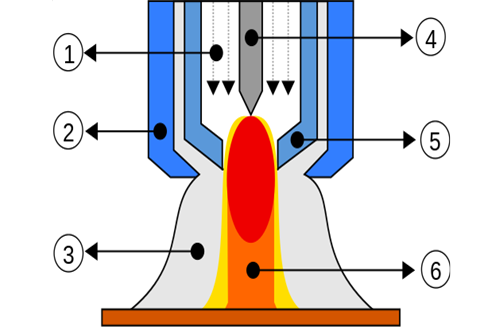
\includegraphics[width=\textwidth]{ptaTorc}
\end{figure}

\subsection{PTA’da kullanılan malzemeler}
PTA işlemi sırasında uygulanan akım, toz besleme hızı, ilerleme hızı ve plazma gaz debisi ortaya çıkan kaplamanın özelliklerini etkilemektedir. Kaplamalarda kullanılan toz malzemelerin ve yukarıda bahsedilen özelliklerin optimum dengede olması PTA kaplamasının istenen özellikleri sağlaması için önemlidir. PTA işlemi ile ilgili özellikler kullanılan kaplama tozuna karar verilmesinden sonra optimize edilmektedir. Kaplama için kullanılacak tozların da çeşitli kısıtları vardır [4]. 
1. Tozun tane boyutu 50µm ile 150µm arasında olmalıdır. Bu sınırların dışındaki tane boyutları besleme sorunlarına sebep olmaktadır. 
2. Toz taneleri küresel ya da keskin köşeli (angular shape) olmalıdır. Fiber tane şekilleri beslemede sorun çıkartmaktadır.
3. Kaplama malzemesi ve kaynak havuzu yakın yoğunlukta olmalıdır. Yüksek yoğunlukta parçacıklar kaynak havuzunda çökme gösterebilir.
